%----------------------------------------------------------------------------------------
%	PACKAGES AND OTHER DOCUMENT CONFIGURATIONS
%----------------------------------------------------------------------------------------

\documentclass[12pt]{article}
\usepackage[english]{babel}
\usepackage[utf8x]{inputenc}
\usepackage{amsmath}
\usepackage{graphicx}
\usepackage[colorinlistoftodos]{todonotes}
\usepackage{booktabs}
\usepackage[numbers]{natbib}
\usepackage{listings}
\usepackage{color}
\usepackage{hyperref}
\usepackage{listingsutf8}
\usepackage{tabularx}
\usepackage{placeins}



 	
% Ruta de las graficas
\graphicspath{{figuras/}}



\begin{document}


\begin{titlepage}

\newcommand{\HRule}{\rule{\linewidth}{0.5mm}} % Defines a new command for the horizontal lines, change thickness here

\center % Center everything on the page
 
%----------------------------------------------------------------------------------------
%	HEADING SECTIONS
%----------------------------------------------------------------------------------------

\textsc{\LARGE Universidad de Antioquia}\\[1.5cm] % Name of your university/college
\textsc{\Large Reporte 3}\\[0.5cm] % Major heading such as course name
% \textsc{\large Reporte 1 - Instalación y configuracion de las herramientas}\\[0.5cm] % Minor heading such as course title

%----------------------------------------------------------------------------------------
%	TITLE SECTION
%----------------------------------------------------------------------------------------

\HRule \\[0.4cm]
{ \huge \bfseries Metricas - Parte 1}\\[0.4cm] % Title of your document
\HRule \\[1.5cm]
 
%----------------------------------------------------------------------------------------
%	AUTHOR SECTION
%----------------------------------------------------------------------------------------

\begin{minipage}{0.4\textwidth}
\begin{flushleft} \large
\emph{Author:}\\
Henry \textsc{Arcila} % Your name
\end{flushleft}
\end{minipage}
~
\begin{minipage}{0.4\textwidth}
\begin{flushright} \large
\emph{Supervisors:} \\
Prof. Natalia \textsc{Gaviria} % Supervisor's Name
Prof. Danny \textsc{Múnera} % Supervisor's Name

\end{flushright}
\end{minipage}\\[2cm]

% If you don't want a supervisor, uncomment the two lines below and remove the section above
%\Large \emph{Author:}\\
%John \textsc{Smith}\\[3cm] % Your name

%----------------------------------------------------------------------------------------
%	DATE SECTION
%----------------------------------------------------------------------------------------

{\large \today}\\[2cm] % Date, change the \today to a set date if you want to be precise

%----------------------------------------------------------------------------------------
%	LOGO SECTION
%----------------------------------------------------------------------------------------


\includegraphics[scale=0.09]{udea_logo4.png}\\[1cm] % Include a department/university logo - this will require the graphicx package
 
%----------------------------------------------------------------------------------------

\vfill % Fill the rest of the page with whitespace

\end{titlepage}

\tableofcontents
\newpage

\begin{abstract}

De a cuerdo a World internet usage and poblation statistics, aproximadamente un 54.4\% tienen acceso a internet \citep{internet_stats}; gracias a esto, son cada vez menores las barreras fisicas para el uso de información. La información es un recurso vital y como tal, debe ser protegido; sin embargo, dicha tarea es cada vez mas desafiante debido a la mayor facilidad, numero y sofisticación de los ataques actualmente existentes. Para hacer frente éstos se han creado diferentes sistemas de seguridad como firewalls, antivirus, IDS e IPS entre otros.

Un sistema de seguridad puede ser visto como una caja negra con unas entradas (datos de red: trafico de red, logs, reportes de hardware), unas salidas (alarmas, reportes de red, logs) y un proceso, cuya finalidad es actuar sobre las entradas, procesarlas y generar las salidas necesarias. Existen muchos tipos de ataques de red siendo los ataques de denegación de servicio unos de los mas comunes. 

Teniendo todo lo anterior y que, la definición y restricción de las entradas de cualquier sistema es vital, el presente reporte tratará las entradas de un sistema de seguridad restringiendo estas solo a ataques de denegación de servicio (DoS) como se mostrará mas adelante. 
 
\end{abstract}

\section{Objetivos}

\begin{enumerate}
\item Describir de manera consista diagrama de bloques de un sistema de seguridad.
\item Hacer un estudio breve de entradas de trafico asociado con ataques de denegacion de servicio.
\item Hacer un inventario a partir de la literatura de algunas metricas del ataque.
\item Cosultar como obtener las metricas.
\end{enumerate}

\section{Introducción}

En la figura 1 de muestra el diagrama de bloques de un sistema de seguridad simplificado que se divide en los siguientes componentes:
\begin{enumerate}
\item \textbf{Preprocesamiento}: Componente que procesa los datos de entrada (datos de red sin procesar) para extraer sus principales caracteristicas con el objetivo de generar una representación equivalente pero mas reducida (vectores caracteristicos) mas apropiada para etapas de procesamiento posteriores.
\item \textbf{Alarma}: este componentes los datos caracteristicos resultantes de la etapa de preproceamiento y lanza alarmas de red (logs que reporta eventos, reportes de red, etc) con el fin de indicar a los administradores posibles problemas en la red. El papel de las alarmas no se limita meramente al de indicadores, tambien pueden ser empleadas como entradas adicionales al componente de procesamiento tal y como se muestra en la figura 1.
\item \textbf{Procesamiento}: este componente lleva a cabo acciones de control (bloquear trafico, limitar ancho de banda, reconfigurar la red, aislar equipos infectados, etc) con el fin de mitigar problemas en la red sin intervención humana.
\end{enumerate}

\begin{figure}[htbp]
\begin{center}
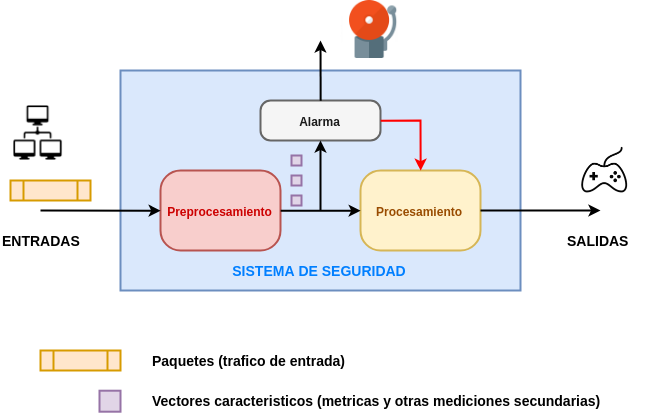
\includegraphics[scale=0.5]{sistema_simplificado2.png}\\[1cm] % Include a department/university logo - this will require the graphicx package
\caption{Sistema de seguridad simplificado}
\end{center}
\end{figure}

En el reporte se hará enfasis en las fuentes empleadas para generar datos de entrada y las diferentes herramientas empleadas para su analisis, restringiendo el estudio a los ataques de denegación de servicio. Finalmente, el documento culminará con una sección dedicada a las discuciones y conclusiones.

\section{Entradas}

Un sistema de seguridad puede procesar diferentes tipos de entradas (trafico de red, carga de memoria, logs, tipo de sistema operativo, puertos abiertos, etc). Existen ademas, diferentes tipos de sistemas de seguridad (antivirus, firewalls, IDS, IPS, etc.) los cuales, de acuerdo a unas entradas determinadas realizan tareas para proteger, desde equipos de computo hasta redes, de ataques. No obstante, el tipo de sistema que se implemente es quien dictará el tipo de entradas que se usen; asi por ejemplo, las entradas para un antivirus no serán las mismas que para un sistema de detección de intruciones (IDS). Lo anterior plantea una primera restricción ¿Que sistema de seguridad se va a implementar?

Para el caso, se hará enfasis en los IDS. Un IDS es un sistema que evalua el tráfico de red en busqueda de amenazas y riesgos y lanza alarmas en caso de deteccion de un patrón de tráfico anormal. 

Una vez definido el sistema en el cual se hará enfasis el siguiente paso, consiste en definir las entradas del sistema que para el caso de los IDS son tráfico de red, sin embargo, ¿como generar trafico de red y mas si se quiere que este sea controlado pues lo que se desea es evaluar bajo condiciones controladas un IDS?

% Introduciendo los ataques DoS como restricción
Como existen diferentes tipos de ataques como herramientas para llevarlos a cabo [dd] es importante tambien definir el tipo de ataque en el cual se hará enfasis; siendo para el caso, el ataque de denegación de servicios (DoS). 

% Halbando de las fuentes de generación de trafico DoS.
 La generación de los datos de entrada (tráfico de red para el caso), 

puede ser hecha empleando las siguientes fuentes:
\begin{itemize}
\item Datasets
\item Herramientas de geneneracion de ataques.
\item Generadores de trafico.
\end{itemize}






\subsection{Fuentes de generación de ataques de degación de servicio}

Cuando nos referimos a las fuentes de generación de ataques, en el siguiente documento queremos hacer referencia a aquellas herramientas y conjuntos de datos que pueden ser empleados como fuente de generacion de trafico no solo para lanzar ataques, sino tambien como sucede mas especificamente en lo que queremos, para evaluar un sistema de seguridad propuesto. Como hablar de ataques es ahondar en un tema muy amplio, la busqueda se restringio a herramientas para lanzar ataques de denegación de servicio para lo cual haciendo una revisión de la literatura se realizo la siguiente clasificación.

\subsubsection{Datasets}

En lo que respecta al trafico de red existen varios datasets (conjunto de datos) relacionados con difentes ataques tales como los que se muestran en la siguiente tabla:

\begin{table}[htbp]
\centering
\begin{tabular}{|p{0.3\linewidth}|p{0.7\linewidth}|}
\hline
\multicolumn{1}{|c|}{\textit{\textbf{Dataset}}} & \multicolumn{1}{c|}{\textit{\textbf{Descripción}}} \tabularnewline \hline
MIT Lincoln Laboratory IDS Datasets \& Scan Data Repository & Large collection of Internet-wide scanning data from Rapid7, the University of Michigan, and others \href{https://scans.io/}{link}  \tabularnewline \hline
UCI & Repositorio de Machine Learnin de la universidad de Irvine \href{https://archive.ics.uci.edu/ml/datasets.html}{link}  \tabularnewline \hline
NSA Cyber Defense Exercise Dataset & Dataset Snort, DNS, web server, and Splunk logs \href{https://www.usma.edu/crc/SitePages/DataSets.aspx}{link} \tabularnewline \hline
Internet-Wide Scan Data Repository & Large collection of Internet-wide scanning data from Rapid7, the University of Michigan, and others \href{https://scans.io/}{link} \tabularnewline \hline
LIBSVM & This page contains many classification, regression, multi-label and string data sets stored in LIBSVM format. Many are from UCI, Statlog, StatLib and other collections \href{https://www.csie.ntu.edu.tw/~cjlin/libsvmtools/datasets/}{link}  \tabularnewline \hline
Center for Applied Internet Data Analysis (CAIDA) Datasets & Internet measurement with collaboration of numerous institutions, academics, commercial and noncommercial contributors, including anonymized Internet traces, Code Red worm propagation, passive traces on high-speed links \href{http://www.caida.org/projects/trends/imdc/}{link} \tabularnewline \hline
\end{tabular}
\end{table}
\FloatBarrier

En cada data set se definen unas parametros (features) como la IP origen, la IP destino, el tipo de ataque, etc. Un ejemplo se puede encontrar en el KDD Cup 1999 Data Set\citep{kdd_desc, CIDDS-001}.

La utilidad de los datasets radica en su amplio uso en areas de investigacion relacionadas con machine learning (ML) y sistemas de intrucion (IDS) \citep{using_kdd} lo que da pie para la utilización de uno de estos dataset con el fin de llevar a cabo la evaluación del sistema de seguridad propuesto. Sin embargo esto abre interrogantes como:
\begin{itemize}
\item ¿Como llevar a cabo un montaje experimental que haga uso de un dataset?
\item ¿Será necesario el uso de todos los parametros de un dataset?, ¿Cuales serian los mas relevantes? 
\item ¿Que se puede lograr empleando un dataset?
\end{itemize}

\subsubsection{Herramientas para lanzar ataques de denegacion de servicio}

Existe un gran numero de herramientas para realizar ataques. Mas exactamente en el caso de los ataques de denegación de servicios, la obtención y uso de estas es sumamente facil gracias a la existencia de portales como \href{http://sectools.org/}{sectools} o distribuciones linux enfocadas en seguridad como kali que traen muchas de estas aplicaciones por defecto. La siguiente tabla \citep{dos_tools} muestran algunas aplicaciones empleadas para lanzar ataques de denegación de servicio de manera resumida:

\begin{table}[htbp]
\centering
\begin{tabular}{|p{0.2\linewidth}|p{0.4\linewidth}|p{0.2\linewidth}|}
\hline
\multicolumn{1}{|c|}{\textit{\textbf{Dataset}}} & \multicolumn{1}{c|}{\textit{\textbf{Descripción}}} & \multicolumn{1}{c|}{\textit{\textbf{Tipo de ataque}}} \tabularnewline \hline
LOIC (Low Orbit Ion Cannon) & herramienta openasource diseñada que
permite realizar ataques de denegacion de servicio enviando un gran cantidad de paquetes de red con el proposito de saturar el ancho de banda & tcp, udp, icmp,http \tabularnewline \hline
HOIC (High Orbit Ion Cannon) & herramienta para lanzar hasta 256 ataques de denegacion (a diferentes dominios) de servicio de manera paralela mediante el envio de GET flood and POST requeststs & http \tabularnewline \hline
HULK (HTTP Unbearable Load King) & herramienta para dar de baja servidores web empleando TCP SYN flood and multi threaded HTTP GET flood requests. Esta herramienta usa varias obfuscation technique para limitar la capacidad del objetivo de mitigar el ataque. & http \tabularnewline \hline
Tor’s Hammer & Es una herramienta escrita en python diseñada para agotar el ancho de banda y los recursos de la victima. Se caracteriza por correr en una red ToR usando direcciones IPs aleatorias con el fin de dificultar el rastreo del atacante. & http \tabularnewline \hline
\end{tabular}
\end{table}



\begin{table}[htbp]
\centering
\begin{tabular}{|p{0.2\linewidth}|p{0.4\linewidth}|p{0.2\linewidth}|}
\hline
\multicolumn{1}{|c|}{\textit{\textbf{Dataset}}} & \multicolumn{1}{c|}{\textit{\textbf{Descripción}}} & \multicolumn{1}{c|}{\textit{\textbf{Tipo de ataque}}} \tabularnewline \hline
RUDY (R-U-dead-Yet) & Es una herramienta escrita en python usada para realizar slow attacks con el fin de comprometer la disponibilidad de servidores web. Los ataques realizados empleando esta herramienta, se caracterizan por abrir conexiones POST HTTP simultáneas un servidor HTTP y, retrazar el envío del cuerpo de la solicitud POST lo cual hace que los recursos del servidor se saturen. El envio pequetes pequeños a un ritmo tan lento (para mantener la conexion abierta y al servidor ocupado) hace que la deteccion de este tipo de ataques sea dificil de detectar comparado con los ataques DoS por inundacion. & http \tabularnewline \hline
Golden-Eye & Es una herramienta escrita en python que permite realizar ataques http flood con el objetivo e agotar los recursos de la victima, es ideal para probar websides pero no es efectiva en el  mundo real los ataques lanzados con esta herramienta son faciles de detectar por defensas perimetrales.  & http \tabularnewline \hline
TFN(Tribe flood network) & es una herramienta con la capacidad de lanzar multiples ataques DDoS usando UDP flood, Smurf attack y TCP SYN flood. & tcp,udp,icmp \tabularnewline \hline
\end{tabular}
\end{table}

\begin{table}[htbp]
\centering
\begin{tabular}{|p{0.2\linewidth}|p{0.4\linewidth}|p{0.2\linewidth}|}
\hline
\multicolumn{1}{|c|}{\textit{\textbf{Dataset}}} & \multicolumn{1}{c|}{\textit{\textbf{Descripción}}} & \multicolumn{1}{c|}{\textit{\textbf{Tipo de ataque}}} \tabularnewline \hline
Slowloris & es una herramienta para lanzar ataques DoS enviando continuamente TCP SYN requests a la victima con el proposito de establecer muchas conexiones abiertas con la victima tanto como sea posible lo que satura la capacidad esta para recibir nuevas conexiones de los clientes. & http \tabularnewline \hline
Ddosim & Es una herramienta para generar ataques DDoS que usa direcciones IP aleatorias para simular varios zombies loc cuales crean conexiones full TCP con la victima. Una vez establecida la conexion la herramienta lanza ataques como HTTP-GET flood para hacerla no disponible. & tcp,smtp ,http,udp \tabularnewline \hline
Pyloris & Esta herramienta permite al usuario realizar ataques DoS sobre un servicio. Puede trabajar con varios protocolos, incluyendo HTTP, FTP, SMTP, IMAP, y Telnet. & --- \tabularnewline \hline
\end{tabular}
\end{table}

\FloatBarrier

Como existen varios tipos de ataques de denegación de servicio; conocer la herramienta, permite definir el tipo de ataque en el que esta se enfoca y por ende es un paso fundamental al definir la entrada que sera empleada en el experimento.

\subsubsection{Generadores de trafico}

Los generadores de trafico son herramientas que pueden generar trafico tanto legitimo como de ataque. A continuación muestran algunos resumiendo sus caracteristicas mas relevantes \citep{dos_tools}. 

\begin{table}[htbp]
\centering
\begin{tabular}{|p{0.1\linewidth}|p{0.5\linewidth}|p{0.1\linewidth}|}
\hline
\multicolumn{1}{|c|}{\textit{\textbf{Generador}}} & \multicolumn{1}{c|}{\textit{\textbf{Descripción}}} & \multicolumn{1}{c|}{\textit{\textbf{Parametros de entrada}}} \tabularnewline \hline
Bit-Twist & Es una herramienta de generacion de diferentes tipos de trafico Ethernet. Permite generar paquetes a partir de trazas tcpdump (.pcap). Adicionalmente, esta herramienta permite la edición de edicion de trazas.  
 & TCP, UDP, IP,ARP \tabularnewline \hline
packETH & Generador de paquetes ethernet que permite crear y enviar cualquier paquete o secuencia de paquetes a traves de un link ethernet.  
 & TCP, UDP, IP, ARP, ICMP \tabularnewline \hline
Nemesis & Utilidad que permite la reacion e inyeccion de paquetes de red. Es ampliamente usado para testear IDS, firewals e IP stacks entre otros.  
 & ARP, DNS, ETHERNET, ICMP, IGMP, IP, OSPF, RIP, TCP, UDP \tabularnewline \hline
D-ITG (Distributed Internet Traffic Generator) & Es una herramienta con la capacidad de generar trafico de manera mas realista usando procesos estocasticos para IDT (Inter Departure Time) y PS (Packet Size).  
 & HTTP, TCP/IP \tabularnewline \hline
curl-loader & Herramienta que simula el comportamiento y carga generada  por miles y decenas de miles de clientes HTTP/HTTPS y FTP/FTPs con sus propias direcciones IP. Esta herramienta es util para la medicion de carfas de desempeño de varias aplicaciones, para testeo de servidores web y ftp y para generar trafico. & HTTP, HTTPS, FTP, FTPS\tabularnewline \hline

\end{tabular}
\end{table}


\begin{table}[htbp]
\centering
\begin{tabular}{|p{0.1\linewidth}|p{0.5\linewidth}|p{0.1\linewidth}|}
\hline
\multicolumn{1}{|c|}{\textit{\textbf{Generador}}} & \multicolumn{1}{c|}{\textit{\textbf{Descripción}}} & \multicolumn{1}{c|}{\textit{\textbf{Parametros de entrada}}} \tabularnewline \hline
HTTPerf & httperf es una herramienta para la medición de desempeño en servidores web. Esta aplicación es basicamente un cliente que ejecuta request especificos contra un servidor para luego realizar mediciones y registros de metricas como el tiempo de resupuesta. & HTTP, SSL \tabularnewline \hline
\end{tabular}
\end{table}






\textbf{Nota}: Ver las herramientas relacionadas ---> http://bittwist.sourceforge.net/doc.html 


\FloatBarrier

Los generadores de trafico son utiles para simular trafido de red, testear firewalls, IDS e IPS, asi mismo para resolver varios problemas de red. (Mejorar esta redaccion y agregar su papel para las entradas)



\section{Analisis de trafico}

\textbf{Herramientas para el monitoreo de trafico}

\begin{table}[htbp]
\centering
\begin{tabular}{|p{0.3\linewidth}|p{0.7\linewidth}|}
\hline
\multicolumn{1}{|c|}{\textit{\textbf{Herramienta}}} & \multicolumn{1}{c|}{\textit{\textbf{Uso}}} \tabularnewline \hline
Wireshark & Analisis de protocolo  \tabularnewline \hline
tcpwrite & Edición de archivos de trafico \textbf{pcap} que permite reescribir headers TCP/IP y de capa 2, asi mismo permite generar trafico mediante el reuso de paquetes \textbf{pcap} ya disponibles. \tabularnewline \hline
tcpreplay &  Permite el reuso de paquetes de trafico previamente capturados a velocidades arbitrarias en la red\tabularnewline \hline
nmap & Herramienta para escaneo de puertos y exploración de redes \tabularnewline \hline
tcptrack & Usada para sniffing y despliegue de información (IPs fuente y destino, estado de la conexion, idle time, Puertos fuente y destino y uso del ancho de banda en la conexion entre otros) de las conexiones de red vistas en la interfaz de red.   \tabularnewline \hline
\end{tabular}
\end{table}



\textbf{Parametros en los paquetes de red - Representación}


Para llevar a cabo la labor de preprocesamiento es necesario hacer una captura de los paquetes que viajan a traves de la red con el proposito de realizar una inspección profunda de sus principales caracteristicas. Interfaces de programación para la captura de paquetes como pcap (packet capture) e interfaces de monitoreo de paquetes como NetFlow o sflow son bastante comunes. La siguiente tabla muestra algunas de las caracteristicas que pueden ser obtenidas con estas:

\begin{table}[htbp]
\centering
\begin{tabular}{|p{0.3\linewidth}|p{0.7\linewidth}|}
\hline
\multicolumn{1}{|c|}{\textit{\textbf{Parametro}}} & \multicolumn{1}{c|}{\textit{\textbf{Descripción}}} \tabularnewline \hline
Src IP & Direccion IP fuente \tabularnewline \hline
Src Port &  Puerto fuente \tabularnewline \hline  
Dest IP & Direccion IP destino \tabularnewline \hline
Dest Port & Puerto destino \tabularnewline \hline
Proto Transport Protocol & Protocolo de transporte  (ICMP, TCP o UDP)  \tabularnewline \hline
Num & Numero del paquete \tabularnewline \hline
Tiempo de llegada & Tiempo de llegada de un paquete \tabularnewline \hline
Size & Tamaño del paquete ??? \tabularnewline \hline
header len & Longitud de la cabecera \tabularnewline \hline
total len & Longitud total (la verdad no se de que???) \tabularnewline \hline
flags & bandereas \tabularnewline \hline
\end{tabular}
\end{table}

\section{Salidas}

\textbf{Extracción de caracteristicas}

El conocimiento de estos parametros de red (algunos de los cuales fueron previamente citados) es de extrema utilidad por que permite analisis de trafico de red tanto offline como online. Sin embargo, adicional a este proceso, es necesario llevar a cabo una tarea adicional sobre el trafico con el fin de seleccionar los parametros mas relevantes u obtener medidas secundarias (metricas) para etapas de procesamiento posteriores. La siguiente tabla muestra algunos de los parametros que suelen ser empleados:

\begin{itemize}
\item \% of same service to same host
\item \% on same host to same service
\item average duration / all services
\item average duration /current host
\item average duration / current service
\item bytes transfered / all services
\item bytes transfered / current host
\item bytes transfered / current service
\item Destination bytes
\item Destination IP
\item Destination port
\item Duplicate ACK rate
\item Duration
\item Hole rate
\item Land packet
\item Protocol
\item Resent rate
\item Source bytes
\item Source IP
\item Source port
\item TCP Flags
\item Timestamp
\item \# different services accessed
\item \# establishment errors
\item \# FIN flags
\item \# ICMP packets
\item \# keys with outside hosts
\item \# new keys
\item \# other errors
\item \# packets to all services
\item \# RST flags
\item \# SYN flags
\item \# to certain services
\item \# to privileged services
\item \# to the same host
\item \# to the same service
\item \# to unprivileged services
\item \# total connections
\item \# unique keys
\item \# urgent
\item \% control packets
\item \% data packets
\item wrong data packet size rate
\item variance of packet count to keys
\end{itemize}

Tras ver todo este gran numero de parametros entran una serie de preguntas que son de vital importancia resolver y que se citan a continuación: 
\begin{itemize}
\item ¿Como obtener todas estas caracteristicas del trafico de red que se esta analizando ya sea de manera online o de manera offline?
\item ¿Que herramientas o librerias pueden existir para facilitar esta tarea?
\item ¿Como configurarlas y ponerlas a punto para la extracción de caracteristicas?
\end{itemize}




\section{Conclusiones}


% https://www.hs-coburg.de/fileadmin/hscoburg/WISENT_cidds_Technical_Report.pdf
% https://www.sans.org/reading-room/whitepapers/detection/security-analytics-fun-splunk-% packet-capture-file-pcap-34580
% https://www.wireshark.org/docs/man-pages/tshark.html
% http://books.gigatux.nl/mirror/snortids/0596006616/toc.html


El código ejemplo se encuentra disponible en: \url{https://github.com/tigarto}

\bibliographystyle{plain}
\bibliography{referencias/bibliografia}


\end{document}